\documentclass[letterpaper,12pt,onehalfspacing,twoside]{article}

\usepackage{lipsum,kantlipsum}
%\usepackage{times}
\usepackage[tmargin=1in,bmargin=1in,lmargin=1in,rmargin=1in]{geometry}
\usepackage{setspace}
%  \spacing{1.5}
\usepackage{float}
\setlength{\parindent}{0pt}
\setlength{\parskip}{1em}
% \setlength{\parskip}{\baselineskip}

\usepackage{verbatim}
\usepackage{titlesec}
% \usepackage{xcolor}
\usepackage{hyperref}
\usepackage{color}
 \definecolor{darkblue}{rgb}{0.0,0.0,0.3}
 \definecolor{lighterblue}{rgb}{0.0,0.0,0.6}
 \definecolor{shade}{gray}{0.8}
 \hypersetup{colorlinks,breaklinks,
            linkcolor=black,urlcolor=darkblue,
            anchorcolor=lighterblue,citecolor=lighterblue}

\usepackage{tikz}
\usetikzlibrary{calc}
\usepackage{eso-pic}
% \usepackage{background}
\usepackage{pdflscape}

\usepackage{titling}
\setlength{\droptitle}{-10em}   % This is your set screw

\usepackage{tfrupee} % Rupee symbol

\usepackage{graphicx}
\usepackage{amsmath} % [fleqn] for left justified % to have only a few equations left justified, crude way is to use \phantom{\hspace{<length>}}
 %\setlength{\mathindent}{0pt} % after the equation. % OR better use what is shown in Chapter8.
\usepackage{amssymb}
% \usepackage{gensymb}
\usepackage[shortlabels]{enumitem}
\usepackage{chemfig}
\usepackage[version=3]{mhchem} % Package for chemical equation typesetting
\usepackage{textcomp}
\usepackage{amsthm} % for theorem-like settings
\usepackage{mathrsfs} % math alphabets

\usepackage{longtable}
\usepackage{caption}
%\usepackage{subfigure}
\usepackage{subfig} % causing problems
\usepackage{tabularx}
\usepackage{decorule}
\usepackage{booktabs} % Allows the use of \toprule, \midrule and \bottomrule in tables for horizontal lines
\usepackage{multirow}
\usepackage{bigstrut}
\usepackage{chngcntr}

\usepackage[titletoc,title]{appendix} % remove titletoc, add toc for another (acceptable??) way of presenting appendices in toc

% \usepackage[nottoc]{tocbibind} %% get NOT numbered bibliography in toc. write [nottoc,numbib] to make it numbered

%\usepackage{tocloft}
%\renewcommand{\printtoctitle}{\centering\Huge\bfseries}
\renewcommand{\contentsname}{\centering \textbf{Table of Contents}}

%% ------------------------HEADER FOOTER SETTINGS------------------------------------------------------------------------------------------------------------

\usepackage{fancyhdr}
\pagestyle{fancy}

%\renewcommand{\sectionmark}[1]{%
% \markright{\thesection\ #1}}
\renewcommand{\sectionmark}[1]{\markright{\thesection.\quad #1}}
\renewcommand{\subsectionmark}[1]{} % eliminates subsection names from headers
\fancyhf{} 
\fancyfoot[RO,LE]{\thepage}
%\fancyfoot[LO,RE]{\it Design a plant to manufacture 500 TPA of N-Methyl J Acid}
\fancyhead[C]{\it\nouppercase\rightmark} % 1. section name

\renewcommand{\headrulewidth}{0pt}
\renewcommand{\footrulewidth}{0pt}
%\addtolength{\headheight}{0.5pt} 
%\fancypagestyle{plain}{%
%\fancyhead{}
%\renewcommand{\headrulewidth}{0pt} % and the line
%}

%% -------------------------THEOREM-LIKE ENVIRONMENT--------------------------------------------------------------------------------------------------------

% \theoremstyle{definition}
% \newtheorem{msdssection}{Section}

\newtheoremstyle{msds} 	          % name
    {\topsep}                    	          % Space above
    {\topsep}                    	          % Space below
    {\normalfont}                           % Body font
    {}                           	          % Indent amount
    {\bfseries\large}                      % Theorem head font
    {.}                          	          % Punctuation after theorem head
    {.5em}                       	          % Space after theorem head
    {}  				          % Theorem head spec (can be left empty, meaning ‘normal’)

\theoremstyle{msds}
\newtheorem{msdssection}{Section}
%  \counterwithin*{msdssection}{subsection}

%% amsthm package documentation for more settings: http://ctan.imsc.res.in/macros/latex/required/amscls/doc/amsthdoc.pdf

%%----------RESET THEOREM COUNTER AFTER EACH \subsection--------------------------------------------------------------------------------------------

\makeatletter
  \@addtoreset{msdssection}{subsection}
\makeatother

%% ------------------------SECTION ALIGNMENT--------------------------------------------------------------------------------------------------------------------




\titleformat*{\section}{\large\bf} % the \titleformat* is short form version. \titleformat gives error because it takes 7 arguments.
\titleformat*{\subsection}{\normalfont\bf}
\titleformat*{\subsubsection}{\normalfont\bf}
% \titleformat*{\subsubsubsection}{\normalfont\bf}

\titlespacing\section{0pt}{0pt plus 0pt minus 2pt}{0pt plus 0pt minus 2pt}
\titlespacing\subsection{0pt}{0pt plus 0pt minus 2pt}{0pt plus 0pt minus 2pt}
\titlespacing\subsubsection{0pt}{0pt plus 0pt minus 2pt}{0pt plus 0pt minus 2pt}

%\titlespacing{\section}{0pt}{\parskip}{-\parskip}
%\titlespacing{\subsection}{0pt}{\parskip}{-\parskip}
%\titlespacing{\subsubsection}{0pt}{\parskip}{-\parskip}

% \setcounter{secnumdepth}{3} % levels under \subsubsection are not numbered
\setcounter{tocdepth}{3}    % levels under \subsubsection are not listed in the TOC

%% -----------------------------------------DEFINE NEW LIST(S)----------------------------------------------------------------------------------------------------------

\newlist{tinylist}{itemize}{3}
    \setlist[tinylist]{label=\textbullet,
			leftmargin=*,
			parsep=0pt,
			topsep=0pt,
			partopsep=0pt,
			itemsep=0pt}

\newlist{smalllist}{itemize}{3}
    \setlist[smalllist]{label=\textbullet,
			leftmargin=*,
			parsep=2pt,
			topsep=0pt,
			partopsep=0pt,
			itemsep=0pt}

%% ----------------------------------------------------------------------------------------------------------------------------------------------------------------------------

%\usepackage[backend=bibtex,url=false,doi=false,isbn=false,style=authoryear,natbib=true]{biblatex} % Uses the bibtex backend with the authoryear citation style (which resembles APA)
% \usepackage[backend=bibtex,url=false,doi=false,isbn=false,style=numeric-comp,sorting=none]{biblatex} % exclude (include) using doi=false (true)

\usepackage{natbib} % [numbers] to get numbers
\usepackage{notoccite}

%\addbibresource{homepaperbib.bib} %% uncomment biblatex package
% \bibliography{Seminar.bib} %% uncomment biblatex package

%% ------------------------------------------------------------------------------------------------------------------------------------------------------
\allowdisplaybreaks
\begin{document}

\pagestyle{plain}

\begingroup  
  \centering
  \LARGE Node-based and flow-based formulations for the Generalized Vehicle Routing Problem
  \\ \large 06-815 Course Project\\
  \large Jay Shah - jrshah@andrew.cmu.edu\par
\endgroup

\section{Introduction}

Several real world situations can be modeled as a GVRP and its special cases. The post-box collection problem described in \citep{Laporte1996} becomes an assymetric GVRP if one or more vehicles are used. The distribution of goods by sea in an archipelago as in Phillippines, New Zealand, Italy, Greece etc. can also be modeled as a GVRP by selecting a number of potential harbors for each island and a fleet of ships is required to visit exactly one harbor for each island.

All calculations were done on a Windows PC with an Intel i7 processor (2.90 GHz).

\section{Definition of the GVRP}

Let $G = (V,A)$ be a directed graph with $V = \{0,1,2,\ldots,n\}$ as the set of vertices and $A = \{(i,j)|i , j \in V , i \ne j\}$ as the set of arcs. A non-negative cost $c_{ij}$ is associated with wach arc $(i,j) \in A$.

The set of vertices $V$ is partitioned into $k + 1$ mutually exclusive subsets (clusters) $V_0, V_1, \ldots, V_k$. The cluster $V_0$ has only one vertex $0$ which represents the depot and the remaining $n$ nodes belong to the remaining $k$ clusters. These can represent geographically distrbuted customers or islands. Each customer has a demand and the demand of each cluster (denoted by $q$) is the total demand of customers in that cluster. The demand of each cluster can be satsfied via any of its vertices. There exist $m$ vehicles, each with capacity $Q$.

The generalized vehicle routing problem (GVRP) consists in finding the minimum total cost tours starting and ending at the depot, such that each cluster should be visited exactly once, the entering and leaving nodes of each cluster is the same and the sum of all the demands of any tour (route) does not exceed the capacity of the vehicle $Q$. An example of a GVRP with a feasible tour is shown in Fig. \ref {fig:example_gvrp}.

\begin{figure}[htbp]
\centering
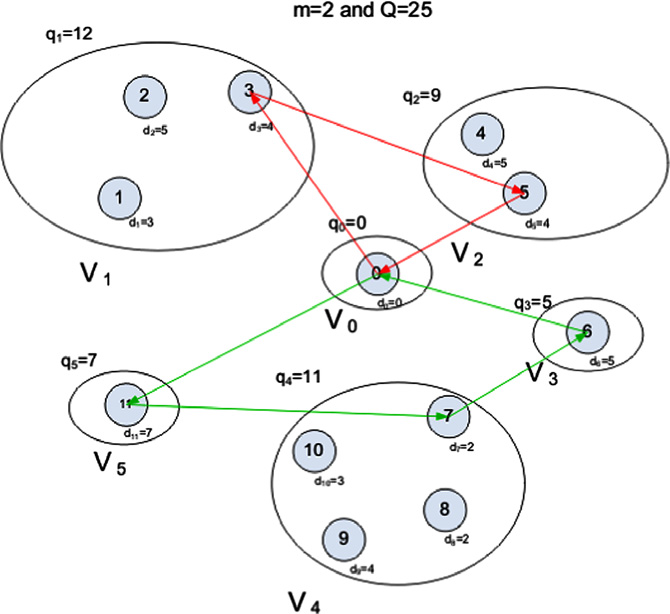
\includegraphics[width=0.6\textwidth]{example_gvrp.png}
\caption{An example of a GVRP and a feasible solution \citep{POP201297}}
\label{fig:example_gvrp}
\end{figure}


\section{MILP formulations}
The first mixed integer linear formulation of the GVRP was presented by \cite{bektasKara} . 


\subsection{General formulation}
The related sets, decision variables and parameters for the GVRP are defined as follows:

\textit{Sets:}

$V = \{0,1,2,\ldots,n\}$ the set of nodes corresponding to the customers, where 0 represents the depot. $V$ is partitioned into mutually exclusive and exhaustive non-empty sub-sets $V_0$, $V_1$, \ldots $V_k$, each of which represents a cluster of customers, where $V_0 = \{0\}$ is the depot.

$K = \{0,1,2,\ldots,k\}$ is the set of clusters.

$A = \{(i,j)|i,j\in V, i\ne j\}$ is the set of arcs.

\textit{Decision variables:}

We define the following binary variables:
\begin{flalign*}
    &x_{ij}= 
\begin{cases}
    1 & \text{if arc $(i,j)$ is included in the tour of a vehicle,  } i \in V_p, j \in V_r, p,r\in K, \\
    0,              & \text{otherwise}
\end{cases} \\
    &W_{pr}= 
\begin{cases}
    1 & \text{if there is a path from cluster $V_p$ to cluster $V_r$,  }  p,r\in K, \\
    0,              & \text{otherwise}
\end{cases}
\end{flalign*}


\textit{Parameters:}

$c_{ij}$ is the cost of traveling from node $i$ to node $j$, $i \ne j$, $i \in V_p$, $j \in V_r$, $p \ne r$, $p,r \in K$;

$d_i$ is the demand of customer $i$, $i = 1,2,\ldots ,n$;

$q_r$ is the demand of the cluster $V_r$, $q_r = \sum_{i \in V_r} d_i$, $r \in K$;

$M = \{1, \ldots,m\}$ is the set of identical vehicles;

$Q$ is the capacity of each vehicle.

We assume that $k \ge m$ ie. the number of vehicles is no greater than the number of clusters.

\subsubsection{Cluster degree constraints}
For each cluster except $V_0$, only a single outgoing arc to any other node belonging to other clusters can exist. This condition is expressed by:
\begin{equation}
\sum_{i \in V_p} \sum_{j\in V \backslash V_p} x_{ij} = 1, p \ne 0, p \in K
\label{cluster1}
\end{equation}
There can be exactly one incoming arc to a cluster from any other node belonging to other clusters, excluding $V_0$. This condition is implied by:
\begin{equation}
\sum_{i \in V \backslash V_p} \sum_{j\in V_p} x_{ij} = 1, p \ne 0, p \in K
\label{cluster2}
\end{equation}
There should be at most $m$ leaving arcs from and at most $m$ entering arcs to the depot:
\begin{flalign}
\sum_{i=1}^n x_{0 i} &\le m \label{cluster3}\\
\sum_{i=1}^n x_{i 0} &\le m \label{cluster4}
\end{flalign}
For the purposes of this study, the constraints \eqref{cluster3} \& \eqref{cluster4} have been taken to be equality constraints.
\subsubsection{Cluster connectivity constraints}
The entering and leaving nodes should be the same for each cluster, which is satisfied by:
\begin{equation}
\sum_{i \in V \backslash V_p} x_{ij} = \sum_{i \in V \backslash V_p} x_{ji}, j \in V_p, p \in K
\label{cluster5}
\end{equation}
Flows from cluster $V_p$ to the cluster $V_r$ are defined by $w_{pr}$. Thus, $w_{pr}$ should be equal to the sum of $x_{ij}$'s from $V_p$ to $V_r$:
\begin{equation}
w_{pr} = \sum_{i \in V_p} \sum_{j \in V_r} x_{ij}
\label{cluster6}
\end{equation}
With the above definitions and constraints, a general integer programming formulation for the GVRP is given as:
\begin{flalign}
\text{min} \; &\sum_{i=1}^n \sum_{j=1}^n c_{ij} x_{ij} \nonumber \\
\text{s.t.} \; & \text{\eqref{cluster1} - \eqref{cluster6}}  \nonumber \\
		  &\text{Capacity bounding constraints} \label{capbound} \\	
		  &\text{Subtour elimination constraints} \label{subtour}\\
		  &x_{i,j} \in \{0,1\}, \forall (i,j) \in A \nonumber
\end{flalign}

We do not need to impose integrality constraints on $w_{pr}$ because Eqs. \eqref{cluster1} - \eqref{cluster4} and \eqref{cluster6} automatically imply that $w_{pr}$ is either $0$ or $1$.

Model formulations of the GVRP are thus constrained by \eqref{cluster1} - \eqref{cluster6} and ``capacity bounding'' and ``subtour elimination'' constraints given in \eqref{capbound} and \eqref{subtour} above.

\cite{POP201297} has presented two different formulations based on additional auxiliary decision variables defined: \emph{node-based} and \emph{flow-based} formulation.

\subsection{Node-based formulation}
In this case, the additional auxiliary variables are defined with respect to the vertices of the graph:

$u_{p}$: the load of a vehicle just after leaving the cluster $V_p$, or delivered amount of goods just after leaving the cluster $V_p$, $p \ne 0$, $p \in K$.








%%%%%
\section{Test examples}

Unfortunately, there is only one test problem for the GVRP given by \cite{GHIANI200011}. This problem (denoted by GVRP1), is originally a VRP taken from \cite{AraqueG1994} with 50 customers and 4 vehicles, with clustering defined by \cite{GHIANI200011}. Each customer has a unit demand and the demand of a cluster is equal to the cardinality of that cluster. 

\subsection{Example 1}
We use the method described above to solve a set of rate equations described by Seinfeld et al. \cite{seinfeld}:
\begin{equation}
\begin{aligned}
&\frac{dy_1}{dt} = - 0.04 y_1 + 10^4 y_2 y_3\\
&\frac{dy_2}{dt} = 0.04 y_1 - 10^4 y_2 y_3 - 3 \cdot 10^7 y_2^2\\
&\frac{dy_3}{dt} = 3\cdot 10^7 y_2^2\\
&y_1(0) = 1, y_2(0) = 0, y_3(0) = 0
\end{aligned}
\end{equation}
The analytical jacobian matrix for this system is given by:
\begin{equation*}
J =\begin{bmatrix}
    -0.04 & 10^4 y_3 & 10^4 y_2  \\
    0.04 & -10^4 y_3 - 6 \cdot 10^7 y_2 & -10^4 y_2 \\
    0 & 6 \cdot 10^7 y_2  & 0
\end{bmatrix}
\end{equation*}
The tolerance vector was taken as $\epsilon = [10^{-3},10^{-7},10^{-3}]$. The integration was carried out in the range [0,10] with an initial step size of $10^{-4}$. The same problem was also solved using \texttt{ode15s}, \texttt{ode23s} and \texttt{ode45}. 

Table \ref{tab:ex1_solvers} shows the statistics involved in computing the solution for the algorithm under consideration and inbuilt MATLAB solvers.  All the three stiff solvers show markedly better performance across all parameters as compared to \texttt{ode45}. The performance of \texttt{ode\_Mic} with an analytical Jacobian is comparable to MATLAB's inbuilt stiff solvers. 
Figure \ref{fig:ex1_solvers} shows the plot of $y_2$ vs time for stiff and non-stiff solutions. We see that the solution using \texttt{ode45} undergoes oscillations at higher time steps.

\begin{figure}[htbp]
\centering
\subfloat[Stiff solver ({\texttt{ode\_Mic}}, \texttt{ode15s} or \texttt{ode23s})]{%
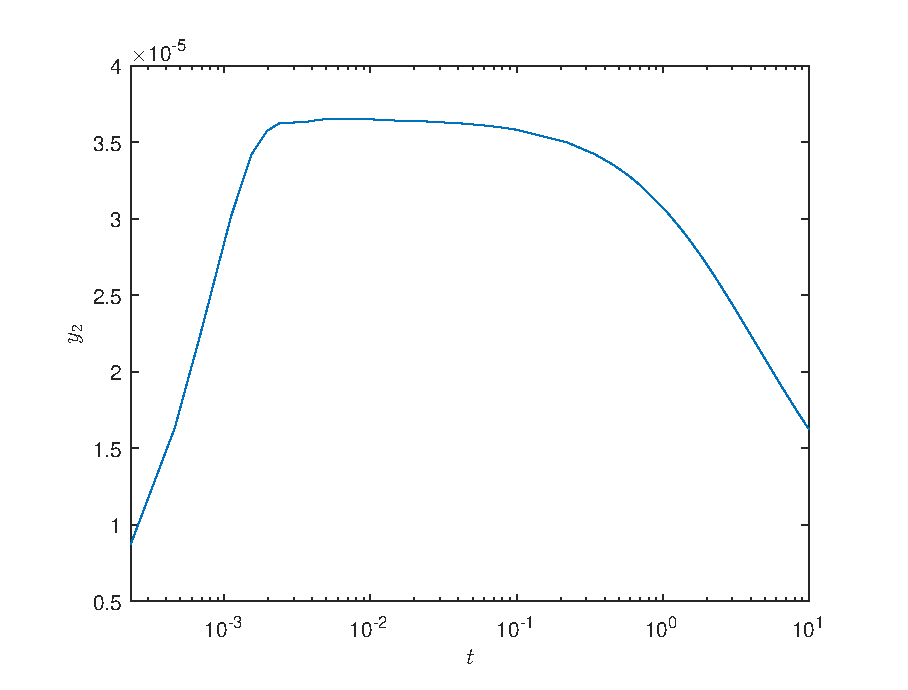
\includegraphics[width=0.45\textwidth]{ode23s.eps}
\label{fig:plot_11}}
\quad
\subfloat[Non-stiff solver (\texttt{ode45})]{%
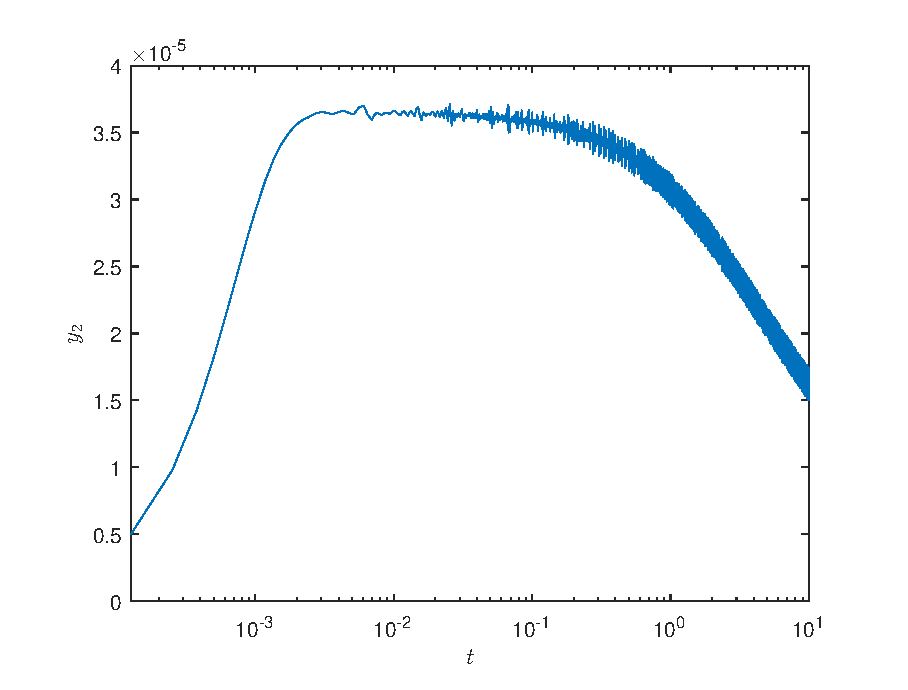
\includegraphics[width=0.45\textwidth]{ode45.eps}
\label{fig:plots_12}}
\caption{Comparision of solutions for non-stiff vs. stiff solvers (Example 1)}
\label{fig:ex1_solvers}
\end{figure}


\begin{table}[htbp]
\centering
\caption{Solver statistics for Michelsen's algorithm compared with inbuilt MATLAB solvers (Example 1)}
\label{tab:ex1_solvers}
\begin{tabular}{@{}llll@{}}
\toprule
                    & Running time (s)  & Function evaluations        & Steps \\ \midrule
                    & \multicolumn{3}{c}{\texttt{ode\_Mic}} \\ \cmidrule(l){2-4} 
Analytical Jacobian & 0.00963       & 168           & 29    \\
Numerical Jacobian  & 0.14337       & 8960          & 29    \\ \cmidrule(l){2-4} 
                    & \multicolumn{3}{c}{\texttt{ode15s}}   \\ \cmidrule(l){2-4} 
Analytical Jacobian & 0.03540      & 81            & 41    \\
Numerical Jacobian  & 0.05238      & 89            & 41    \\ \cmidrule(l){2-4} 
                    & \multicolumn{3}{c}{\texttt{ode23s}}   \\ \cmidrule(l){2-4} 
Analytical Jacobian & 0.00851      & 60            & 19    \\
Numerical Jacobian  & 0.01168      & 115           & 19    \\ \cmidrule(l){2-4} 
                    & \multicolumn{3}{c}{\texttt{ode45}}    \\ \cmidrule(l){2-4} 
 		       & 1.20454      & 52201  & 29109 \\ \bottomrule
\end{tabular}
\end{table}

\subsection{Example 2}
The second test example is a model for a fluid bed reactor \citep{AIC:AIC690200225}:
\begin{equation}
\begin{aligned}
&\frac{dy_1}{dt} = 1.30 (y_3 - y_1) + 1.04 \cdot 10^4 k y_2\\
&\frac{dy_2}{dt} = 1.88 \cdot 10^3 (y_4 - y_2 (1 + k))\\
&\frac{dy_3}{dt} = 1752 + 266.7 y_1 - 269.3 y_3\\
&\frac{dy_4}{dt} = 0.1 + 320 y_2 - 321 y_4\\
&y_1(0) = 759.167, y_2(0) = 0, y_3(0) = 600, y_4(0) = 0.1
\end{aligned}
\end{equation}
where $k = 0.0006 \exp{(20.7 - 15000/y_1)}$. 

The tolerance vector was taken as $\epsilon = [1,1,0.1,0.1]$. The integration was carried out in the range [0,500] with an initial step size of $10^{-4}$. Similar to Example 1, the running time of \texttt{ode\_Mic} with a Numerical Jacobian was comparable to that of \texttt{ode15s} and \texttt{ode23s} (Table \ref{tab:ex2_solvers}). The performance of \texttt{ode45} is several orders of magnitude worse than the stiff solvers.

\begin{table}[htbp]
\centering
\caption{Solver statistics for Michelsen's algorithm compared with inbuilt MATLAB solvers (Example 2)}
\label{tab:ex2_solvers}
\begin{tabular}{@{}llll@{}}
\toprule
                    & Running time (s)   & Function evaluations    & Steps    \\ \midrule
                    & \multicolumn{3}{c}{\texttt{ode\_Mic}} \\ \cmidrule(l){2-4} 
Analytical Jacobian  & 0.014103       & 252       & 43       \\
Numerical Jacobian & 0.341434       & 16112     & 39       \\ \cmidrule(l){2-4} 
                    & \multicolumn{3}{c}{\texttt{ode15s}}   \\ \cmidrule(l){2-4} 
Analytical Jacobian  & 0.190613       & 2354      & 764      \\
Numerical Jacobian & 0.02084        & 126       & 85       \\ \cmidrule(l){2-4} 
                    & \multicolumn{3}{c}{\texttt{ode23s}}   \\ \cmidrule(l){2-4} 
Analytical Jacobian  & 0.018893       & 341       & 114      \\
Numerical Jacobian & 0.014007       & 331       & 48       \\ \cmidrule(l){2-4} 
                    & \multicolumn{3}{c}{\texttt{ode45}}    \\  \cmidrule(l){2-4} 
	 	       & 55.881972      & 2123530   & 1327201  \\ \bottomrule
\end{tabular}
\end{table}

\subsection{Example 3 - Oregonator reaction}
The oscillatory reaction between \ce{H Br O2}, \ce{Br-} and Ce(IV) is known as the Oregonator reaction \citep{oregonator}. The rate expressions are given by:
\begin{equation}
\begin{aligned}
&\frac{dy_1}{dt} = 77.27 (y_2 + y_1(1 - 8.375 \times 10^{-6} y_1 - y_2))\\
&\frac{dy_2}{dt} = \frac{1}{77.27} (y_3 - (1 + y_1) y_2)\\
&\frac{dy_3}{dt} = 0.161 (y_1 - y_3)\\
&y_1(0) = 1, y_2(0) = 2, y_3(0) = 3
\end{aligned}
\end{equation}
\begin{figure}[htbp]
\centering
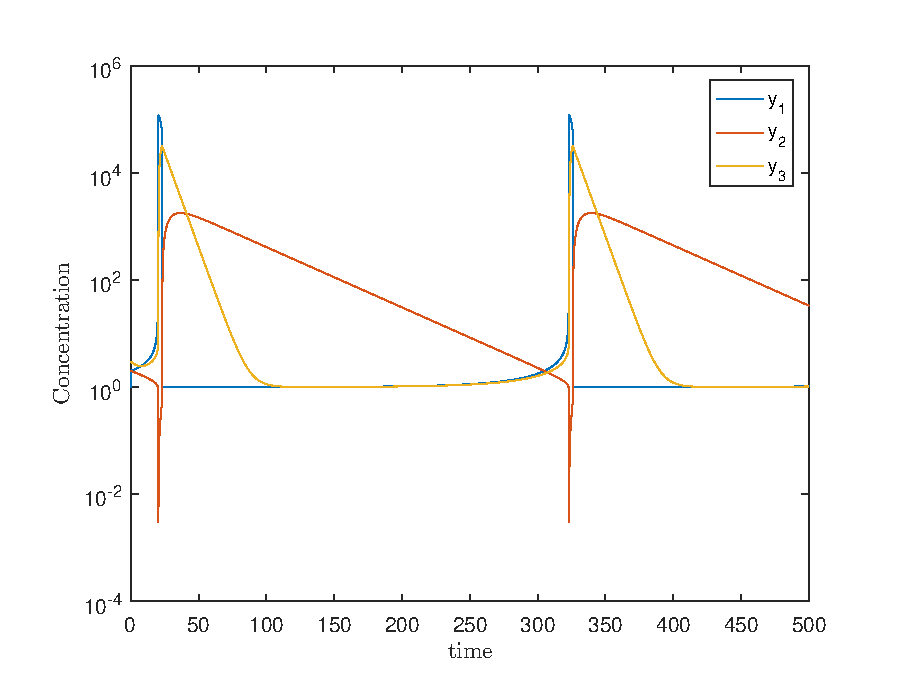
\includegraphics[width=0.6\textwidth]{oregonator.eps}
\caption{Oregonator reaction plot}
\label{fig:ex3_solvers}
\end{figure}
In this system, we observe that at smaller integration limits (e.g. [0,10]) the problem is non-stiff and both stiff and non-stiff solvers integrate the system effectively. However, at larger intervals (once oscillations start taking place), the stiff solvers show markedly better performance than \texttt{ode45} (Table \ref{tab:ex3_solvers}).
 
\begin{table}[htbp]
\centering
\caption{Solver statistics for Michelsen's algorithm compared with inbuilt MATLAB solvers (Example 3 - Oregonator reaction)}
\label{tab:ex3_solvers}
\begin{tabular}{llll}
\hline
                    & Running time  & Function evaluations    & Steps     \\ \hline
                    & \multicolumn{3}{c}{\texttt{ode\_Mic}} \\ \cmidrule(l){2-4} 
Analytical Jacobian & 0.15919      & 5538      & 923       \\
Numerical Jacobian  & 4.46163      & 295203    & 923       \\ \cmidrule(l){2-4} 
                    & \multicolumn{3}{c}{\texttt{ode15s}}   \\ \cmidrule(l){2-4} 
Analytical Jacobian & 0.11093      & 1566      & 583       \\
Numerical Jacobian  & 0.11796      & 1845      & 583       \\ \cmidrule(l){2-4} 
                    & \multicolumn{3}{c}{\texttt{ode23s}}   \\ \cmidrule(l){2-4} 
Analytical Jacobian & 0.06939      & 2142      & 709       \\
Numerical Jacobian  & 0.14239       & 4266      & 709       \\ \cmidrule(l){2-4} 
                    & \multicolumn{3}{c}{\texttt{ode45}}    \\ \cmidrule(l){2-4} 
		       & 584.78864     & 28648200  & 17905633  \\ \hline
\end{tabular}
\end{table}

\newpage
\subsection{Example 4 - Photochemical smog model}

A kinetic model Photochemical smog formation presented by Gelinas \citep{GELINAS1972222} is solved. The original model given in ref.~\citep{GELINAS1972222} involves 29 species and over 60 equations with rate constants varying by 20 orders of magnitude. A simplified form of the model as described in ref. \citep{MICHELSEN1977107} with 12 species and 22 reactions is used and shown in Tables \ref{tab:smog_components} \& \ref{tab:smog}. 

The system was solved using \texttt{ode\_Mic}, \texttt{ode15s}, \texttt{ode23s} and \texttt{ode45} for increasing integration limits. As expected  (especially for this large system), \texttt{ode45} is orders of magnitude worse than any of the stiff solvers for all integration limits. Interestingly, \texttt{ode45} varies as $\mathcal{O}(n)$  whereas \texttt{ode\_Mic} varies as $\mathcal{O}(n^{0.5})$ (where $n$ is max integration limit). 
\begin{table}[H]
\centering
\caption{Components in the smog model}
\label{tab:smog_components}
\begin{tabular}{@{}lll@{}}
\toprule
1. \ce{NO2} & 2. \ce{NO}        & 3. \ce{O}        \\
4. \ce{O3}  & 5. \ce{C4H8}      & 6. \ce{C3H7O2}   \\
7. \ce{HO2} & 8. \ce{CH3CO3}    & 9. \ce{CH3O2}  \\
10. \ce{HO} & 11. \ce{C4H8OHO2} & 12. \ce{CH2OHO2} \\ \bottomrule
\end{tabular}
\end{table}


\begin{table}[H]
\centering
\caption{Photochemical smog model (Example 3) - Reactions and rate constants.}
\label{tab:smog}
\begin{tabular}{@{}ccccccccc@{}}
\toprule
1 &   &    & $\longrightarrow$ & 2        & +       & 3       &  & 6.7 $\times$ 10$^{-\text{3}}$   \\
3 &   &    & $\longrightarrow$ & 4        &         &         &  & 6.73 $\times$ 10$^{\text{4}} $  \\
2 & + & 4  & $\longrightarrow$ & 1        &         &         &  & 9.1  $\times$ 10$^{-\text{2}}$  \\
3 & + & 5  & $\longrightarrow$ & 6        & +       & 7       &  & 3.8 $\times$ 10$^{\text{2}}  $   \\
6 & + & 2  & $\longrightarrow$ & 1        & +       & 7       &  & 3.0       \\
4 & + & 5  & $\longrightarrow$ & 7        & +       & 8       &  & 4.9 $\times$ 10$^{-\text{5}}$\\
4 & + & 5  & $\longrightarrow$ & 4        &         &         &  & 2.1 $\times$ 10$^{-\text{5}}$\\
2 & + & 8  & $\longrightarrow$ & 1        &    +    & 9       &  & 3.0        \\
1 & + & 8  & $\longrightarrow$ & \multicolumn{3}{l}{inactive} &  & 0.1      \\
5 & + & 8  & $\longrightarrow$ & 9        &         &         &  & 1.0 $\times$ 10$^{-\text{4}}  $\\
2 & + & 9  & $\longrightarrow$ & 1        & +       & 7       &  & 3.0        \\
5 & + & 10 & $\longrightarrow$ & 11       &         &         &  & 1.0 $\times$ 10$^{\text{2}}   $   \\
2 & + & 11 & $\longrightarrow$ & 1        & +       & 12      &  & 3.0       \\
2 & + & 12 & $\longrightarrow$ & 1        & +       & 10      &  & 3.0     \\
2 & + & 7  & $\longrightarrow$ & 1        & +       & 10      &  & 50       \\
7 & + & 7  & $\longrightarrow$ & \multicolumn{3}{l}{inactive} &  & 50       \\
7 & + & 10 & $\longrightarrow$ & \multicolumn{3}{l}{inactive} &  & 50       \\
7 & + & 6  & $\longrightarrow$ & \multicolumn{3}{l}{inactive} &  & 50       \\
7 & + & 9  & $\longrightarrow$ & \multicolumn{3}{l}{inactive} &  & 50       \\
7 & + & 8  & $\longrightarrow$ & \multicolumn{3}{l}{inactive} &  & 50       \\
7 & + & 11 & $\longrightarrow$ & \multicolumn{3}{l}{inactive} &  & 50       \\
7 & + & 12 & $\longrightarrow$ & \multicolumn{3}{l}{inactive} &  & 50       \\ \bottomrule
\end{tabular}
\end{table}

\begin{table}[H]
\centering
\caption{Solver statistics for Michelsen's algorithm compared with inbuilt MATLAB solvers (Example 4 - smog model)}
\label{tab:smog_stat}
\begin{tabular}{@{}llll@{}}
\toprule
Time step (s) & Running time (s) & Function evaluations & Steps   \\ \midrule
                    & \multicolumn{3}{c}{\texttt{ode\_Mic}} \\ \cmidrule(l){2-4} 
1        & 1.010029     & 15072                & 13      \\
10       & 3.025674     & 51496                & 42      \\
100      & 8.835829     & 158262               & 126     \\
1000     & 25.085625    & 456571               & 362     \\ \cmidrule(l){2-4} 
                    & \multicolumn{3}{c}{\texttt{ode15s}} \\ \cmidrule(l){2-4} 
1        & 0.021004     & 61                   & 26      \\
10       & 0.060441     & 146                  & 48      \\
100      & 0.085993     & 233                  & 75      \\
1000     & 0.034693     & 284                  & 94      \\ \cmidrule(l){2-4} 
                    & \multicolumn{3}{c}{\texttt{ode23s}} \\ \cmidrule(l){2-4} 
1        & 0.083637     & 252                  & 17      \\
10       & 0.057533     & 569                  & 38      \\
100      & 0.081612     & 914                  & 61      \\
1000     & 0.104977     & 1259                 & 84      \\ \cmidrule(l){2-4} 
                    & \multicolumn{3}{c}{\texttt{ode45}} \\ \cmidrule(l){2-4} 
1        & 6.104102     & 137725               & 86245   \\
10       & 67.269395    & 1379530              & 862373  \\
100      & 653.744277   & 13792100             & 8620221 \\ \bottomrule
\end{tabular}
\end{table}

\section{Conclusion}

The integration algorithm proposed by Michelsen was implemented and found to be well suited for a variety of stiff problems arising in chemical engineering. Using the analytical Jacobian improves performance in each of the stiff solvers used. In all these cases, an arbitrary initial step size was chosen. A more systematic method may improve performance by reducing the number of step length adjustments required for the first step.

\newpage

\nocite{*}  %% uncomment to include all references in bib file
\bibliographystyle{ICTv3}
\bibliography{Proposal_bib}

\end{document}